
\section{Pipeline}
We describe the pipeline $p$ that we run on each text $T$. The pipeline
consists of multiple natural language annotators that we run in 
the sequence outlined below.
\citep{manning2014stanford}
\subsection{Tokenizer}
\subsection{Sentence Splitter}
\subsection{Part of Speech}

\begin{figure}
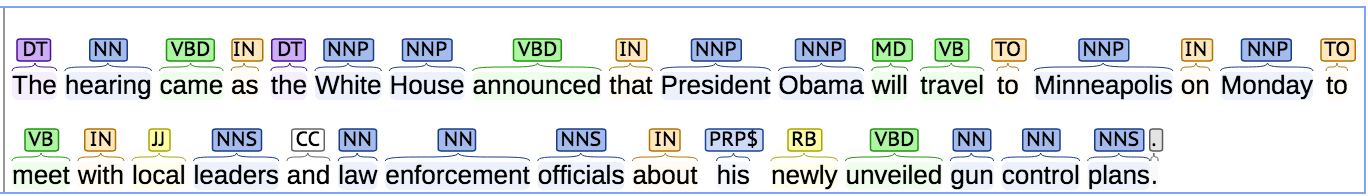
\includegraphics[scale=0.33]{figures/pos.png}
\caption{
\label{fig:pos}
Part of Speech tags on example sentence.
}
\end{figure}

\citet{toutanova2003tagger}
\subsection{Named Entity Recognition}

\begin{figure}
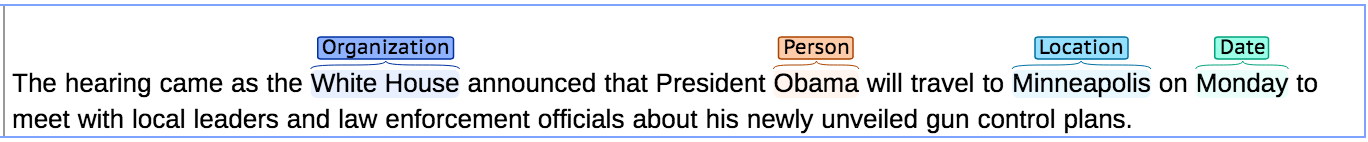
\includegraphics[scale=0.33]{figures/ner.png}
\caption{
\label{fig:ner}
Named Entity Recognition on example sentence.
}
\end{figure}

\citet{finkel2005incorporating}
\subsection{Dependency Parse}

\begin{figure}
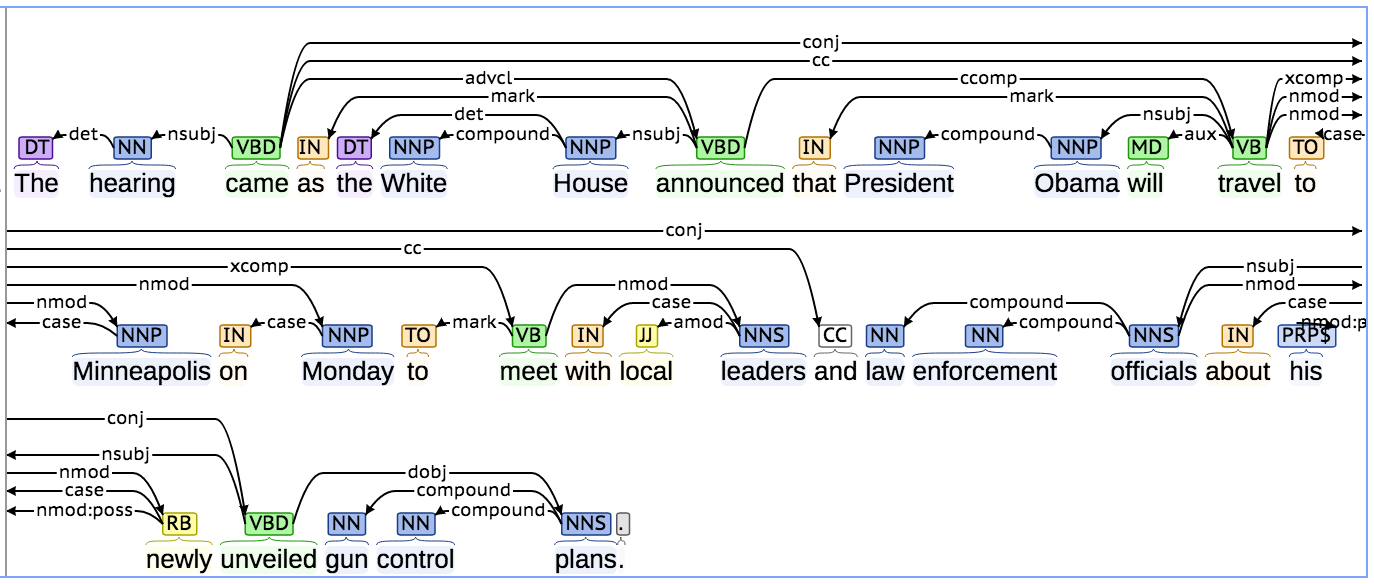
\includegraphics[scale=0.33]{figures/dep.png}
\caption{
\label{fig:dep}
Dependency parse on example sentence.
}
\end{figure}

\citet{chen2014nndep}
\subsection{Mention Resolver}

\subsection{Natural Logic Resolver}
\subsection{Coreference Resolution}

\begin{figure}
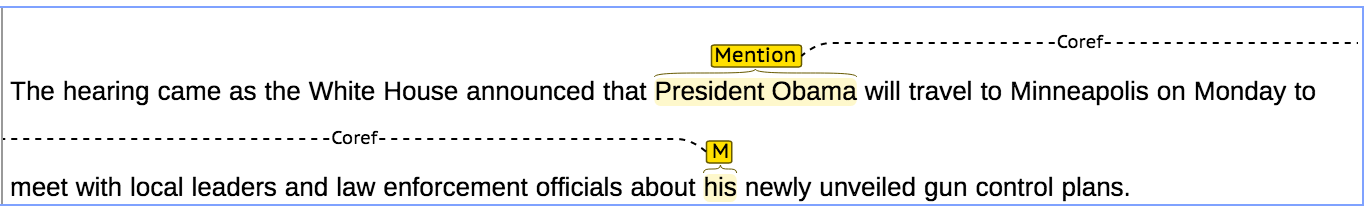
\includegraphics[scale=0.33]{figures/coref.png}
\caption{
\label{fig:coref}
Coreference resolution on example sentence.
}
\end{figure}

\citet{clark2015coref}

\section{Relation Extractor}
Limit max number of entailments taken per clause to 100.
\citet{angeli2015openie}
\citet{fader11reverb}

\subsection{With Coreference Resolution}

\subsection{Without Coreference Resolution}
